% multiple1902 <multiple1902@gmail.com>
% intro.tex
% Copyright 2011~2012, multiple1902 (Weisi Dai)
% https://code.google.com/p/xjtuthesis/
%
% It is strongly recommended that you read documentations located at
%   http://code.google.com/p/xjtuthesis/wiki/Landing?tm=6
% in advance of your compilation if you have not read them before.
%
% This work may be distributed and/or modified under the
% conditions of the LaTeX Project Public License, either version 1.3
% of this license or (at your option) any later version.
% The latest version of this license is in
%   http://www.latex-project.org/lppl.txt
% and version 1.3 or later is part of all distributions of LaTeX
% version 2005/12/01 or later.
%
% This work has the LPPL maintenance status `maintained'。
%
% The Current Maintainer of this work is Weisi Dai。
%

\chapter{基于边缘骨架切割的文字检测方法}
\echapter{Text detection based on Skeleton-cut detector}

    \section{问题的提出}
    \esection{Questions Posed}

    \section{方法原理与步骤}
    \esection{Principle and Summary of The Method}

    基于边缘骨架切割的文字检测子的具体流程如图\ref{fig.c3_overview} 所示。首先对于输入的场景文字图片,利用结构化边缘检测方法\cite{Dollar2015Fast} 得到输入图片的结构化边缘响应图,如图\ref{fig.c3_overview}(b) 所示。然后基于一系列像素强度值阈值,对边缘响应图进行分割,得到相应的二值化边缘图。接着在每个二值边缘图上,通过细化操作得到其边缘骨架图,如图\ref{fig.c3_overview}(c) 所示。图中的红色结点是在边缘骨架上,通过8领域内像素点分析所找到的边缘骨架结点。而文字边缘与背景间的粘连点,就存在于这些边缘骨架结点中。
    为了将文字边缘从背景杂质中切割出来,需要切割开这些边缘骨架结点,以解决文字边缘的粘连问题。而由不同的二值边缘图所生成的边缘骨架图上的结点是不同的。因此选择合适的边缘骨架图上的结点进行切割,是解决文字边缘粘连问题的核心步骤。

    \begin{figure*}[htbp]
    \centering
    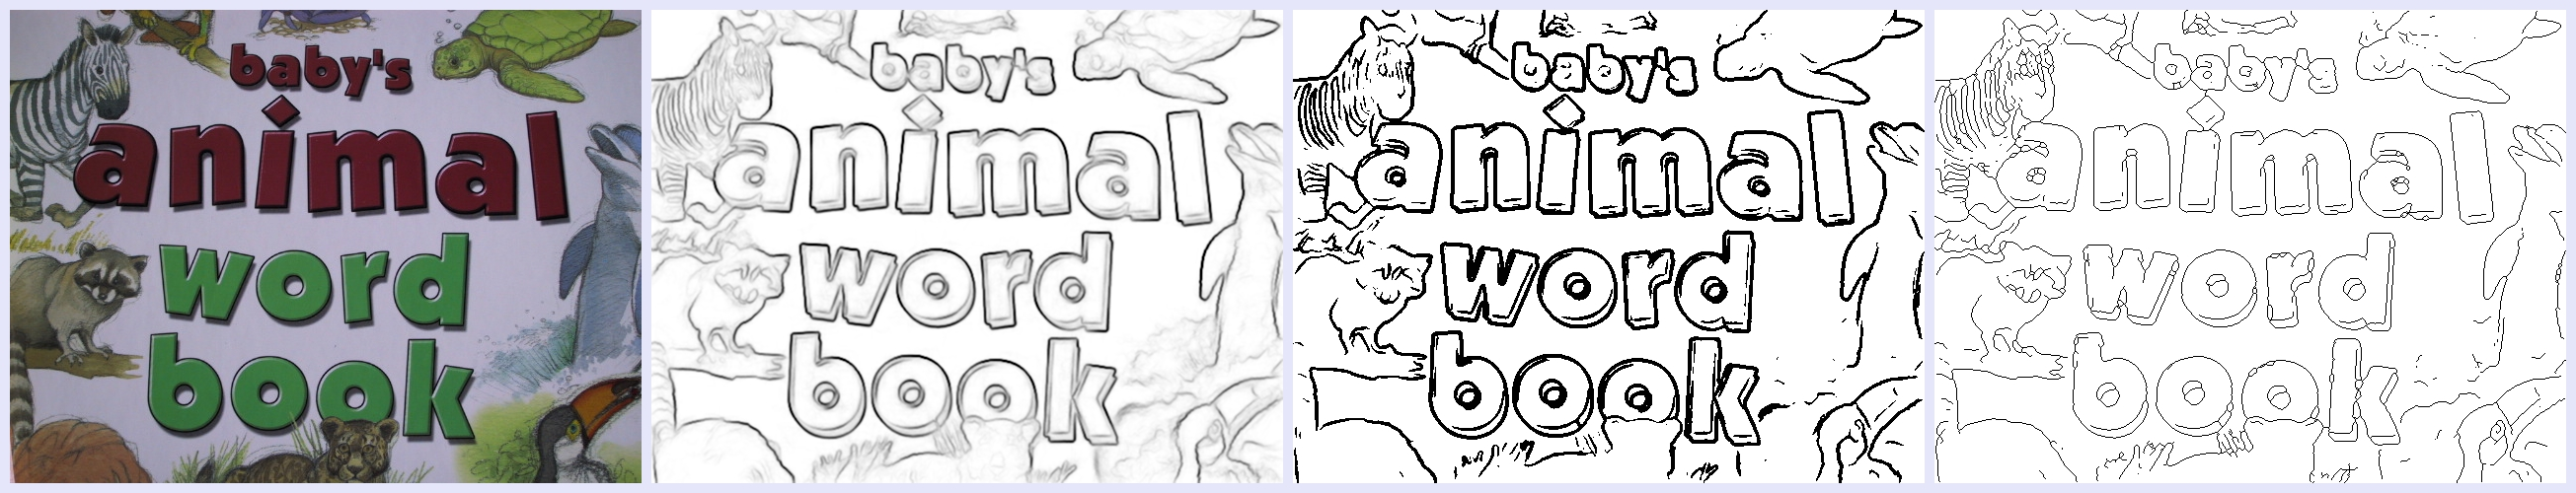
\includegraphics[width=\textwidth]{./figures/c3_overview_1.jpg}
    \begin{minipage}[t]{0.22\linewidth}
    \centerline{ \small (a)输入场景文字图}
    \end{minipage}
    \begin{minipage}[t]{0.22\linewidth}
    \centerline{ \small (b)边缘响应}
    \end{minipage}
    \begin{minipage}[t]{0.22\linewidth}
    \centerline{ \small (c)边缘二值图}
    \end{minipage}
    \begin{minipage}[t]{0.22\linewidth}
    \centerline{ \small (d)边缘骨架}
    \end{minipage}
    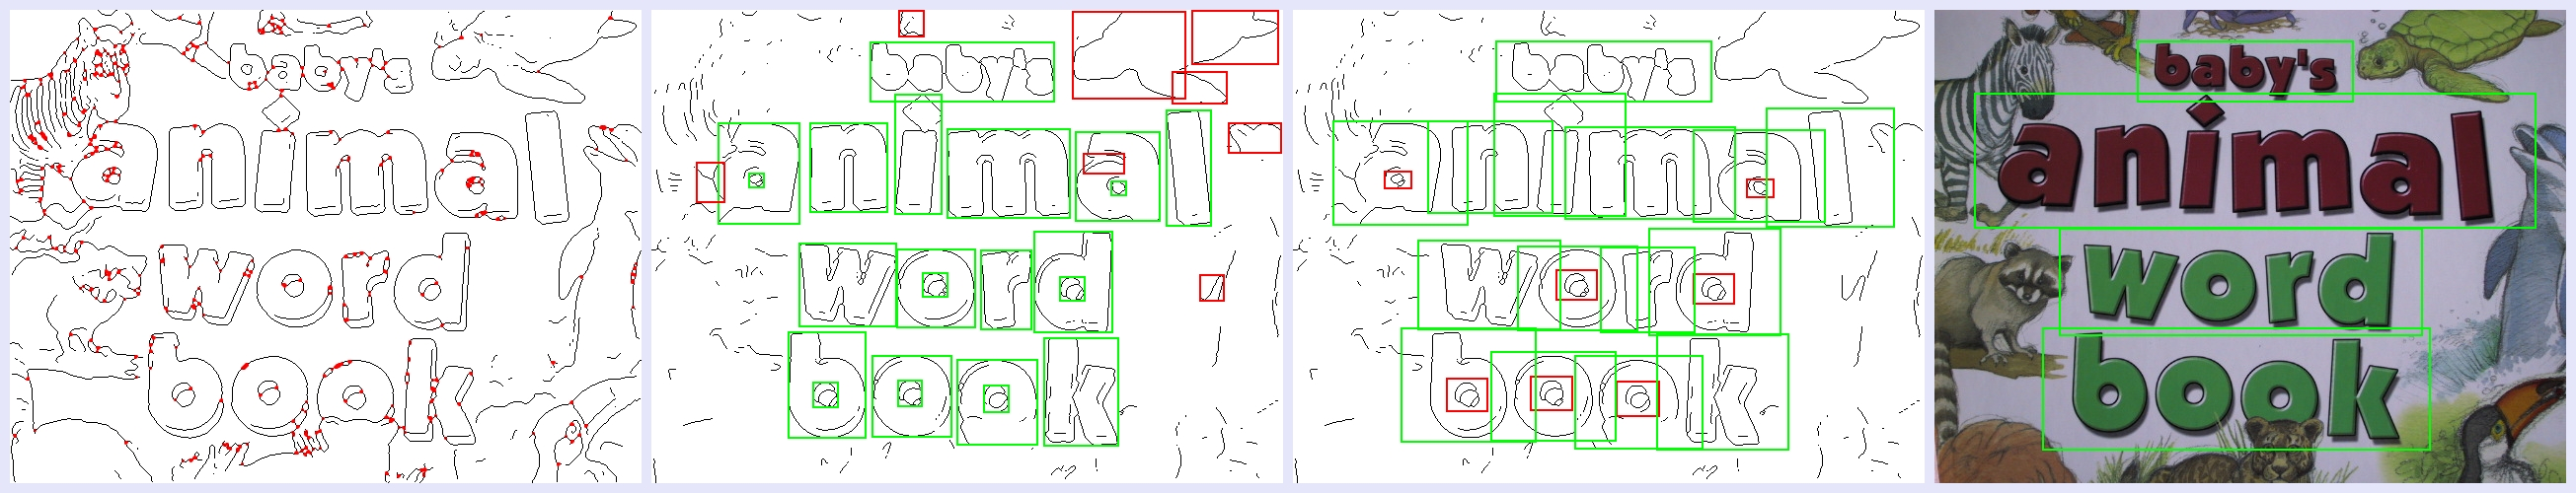
\includegraphics[width=\textwidth]{./figures/c3_overview_2.jpg}
    \begin{minipage}[t]{0.22\linewidth}
    \centerline{ \small (e)边缘骨架切割}
    \end{minipage}
    \begin{minipage}[t]{0.22\linewidth}
    \centerline{ \small (f)非文字骨架的滤除}
    \end{minipage}
    \begin{minipage}[t]{0.22\linewidth}
    \centerline{ \small (g)文本行生成}
    \end{minipage}
    \begin{minipage}[t]{0.22\linewidth}
    \centerline{ \small (h)文字粗略定位结果}
    \end{minipage}
    \caption{基于边缘骨架切割的文字检测方法的流程图}
    \label{fig.c3_overview}
    \end{figure*}

    这里通过实验观察可知,那些分割阈值较低所得的二值边缘图所生成的边缘骨架较为杂乱,更可能是无效的边缘骨架,如图\ref{fig.c3_select_skeleton}(a) 所示。
    因此这里采用欧拉数计算,来从一系列边缘骨架图中选择出最合适的边缘骨架图,欧拉数的计算过程如图\ref{fig.c3_select_skeleton}(b) 所示。在边缘骨架图中,所有的候选边缘骨架都要经过形态学滤除,以过滤掉大部分明显不是文字的边缘骨架。该滤除过程如图\ref{fig.c3_overview}(c)到图\ref{fig.c3_overview}(d) 的变化所示。紧接着,剩余的不易区分的非文字边缘骨架,可通过基于CNN的分类器来进一步滤除。该滤除过程如图\ref{fig.c3_overview}(d)到图\ref{fig.c3_overview}(e)所示,红色框中包含的不易区分的非文字边缘骨架,可通过CNN 分类器去除掉。最后如图\ref{fig.c3_overview}(f)所示,基于非极大值抑制和文本行聚集操作,得到粗略的文本行定位结果。

    \section{文字骨架的提取与切割}
    \esection{Text skeleton's extraction and cutting}

        \subsection{文字骨架的生成}
        \esubsection{Text skeleton's construction}
        \label{sec.c3_skeleton}

        %一系列分割阈值,得到不同的二值边缘图,并生成相应的边缘骨架图;低分割阈值的二值图所生成骨架图较为杂乱,不适合用于后续的边缘骨架切割步骤;这部分内容在supplement 上有,将其作图写在skeleton 的生成一节中。

        在输入的场景文字图像上,通过结构化边缘检测子\cite{Dollar2015Fast} 得到了图像的结构化边缘响应图。边缘响应图并不是二值图,其每个位置上的像素点的值代表的是该像素点属于边缘的概率。如图\ref{fig.c3_overview}(b) 所示,某位置的像素点的值越大,图中该位置的像素点的颜色就越深,说明该位置的像素点越可能位于一条边缘之上。既然边缘响应图是每个位置像素点的值都不尽相同的概率图,为了便于观察,用图\ref{fig.c3_response_to_map}第一行的三维图展示其概率响应。然后按照一系列像素灰度值阈值,对边缘响应图进行分割,得到相应阈值下的二值边缘图。这些二值边缘图如图\ref{fig.c3_response_to_map}中第二行所示。

        从图\ref{fig.c3_response_to_map} 中可以看出,当分割阈值较小时,从边缘响应图上分割得到的二值边缘图较为清晰,但存在大量非文字的边缘,导致文字边缘与背景的粘连问题较为严重。而当分割阈值较大时,从边缘响应图上分割得到的二值边缘图中,大部分非文字的边缘已经被略去,而文字边缘相对而言被较为完整的保留下来,使得文字边缘的粘连问题得到缓解。但同时,大阈值分割下的二值边缘图较为模糊和残缺,边缘时有断裂现象,不利于后续的边缘分析与处理。

        \begin{figure*}[htbp]
        \centering
        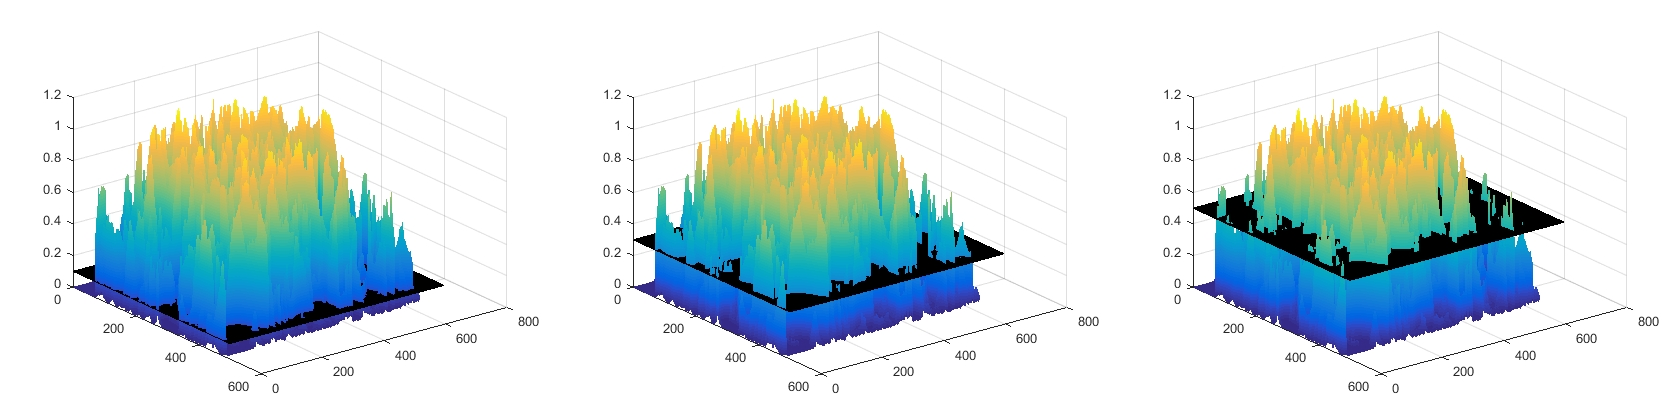
\includegraphics[width=\textwidth]{./figures/c3_edge_response.jpg}
        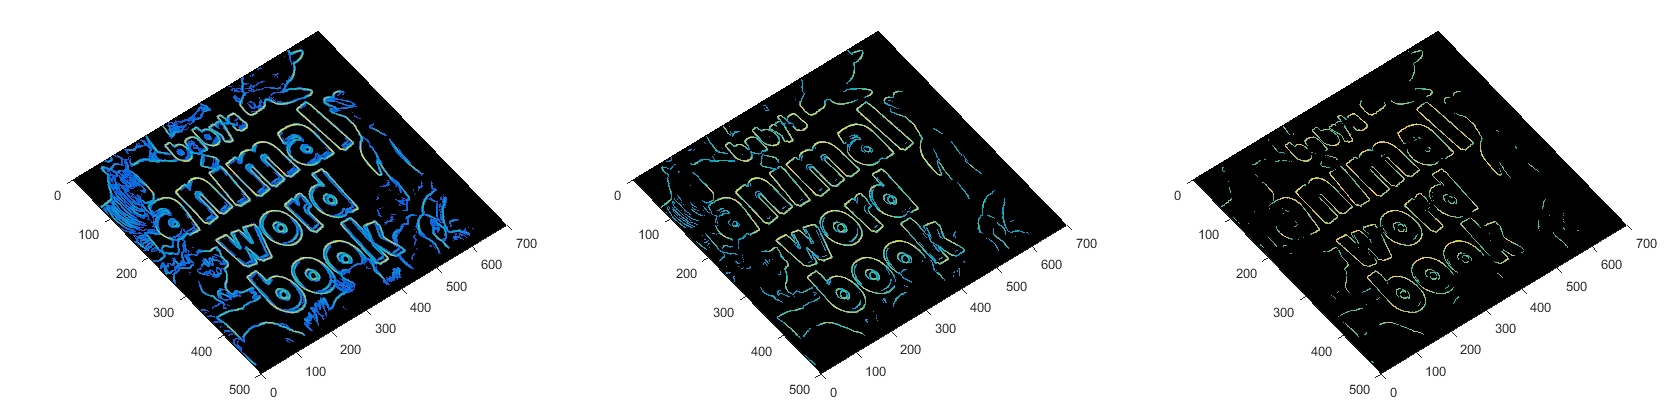
\includegraphics[width=\textwidth]{./figures/c3_edge_map.jpg}
        \begin{minipage}[t]{0.32\linewidth}
        \centerline{ \small (a)阈值 $t = 0.1$}
        \end{minipage}
        \begin{minipage}[t]{0.32\linewidth}
        \centerline{ \small (b)阈值 $t = 0.3$}
        \end{minipage}
        \begin{minipage}[t]{0.32\linewidth}
        \centerline{ \small (c)阈值 $t = 0.5$}
        \end{minipage}
        \caption{在边缘响应图上通过一系列的分割阈值得到相应的边缘二值图}
        \label{fig.c3_response_to_map}
        \end{figure*}

        因此,分割阈值不同,从边缘响应图上分割得到的二值边缘图也不同。较高阈值下的边缘图保留了更多的边缘信息,但更难区别文字与非文字边缘。较低阈值的边缘图去除了非文字边缘信息,但边缘更不清晰。不同于Canny算子\cite{Ding2001On} 等固定阈值的边缘二值图检测方法,本文采用递增的分割阈值从边缘响应图中得到一系列候选边缘二值图,然后从中自适应地选择出最合适的二值边缘图进行后续处理。自适应选择最优二值边缘图的内容会在\ref{sec.c3_skeleton_cut}节中详细阐述。

        接下来利用8连通区域细化方法\cite{Lam2002Thinning} 在二值边缘图上提取边缘的骨架线。该细化方法会一直重复迭代操作,直到图像不再发生变化。每次迭代操作包含2个子迭代操作:在第1个子迭代操作中,当且仅当条件 $G_1$, $G_2$ 和 $G_3$全部满足时,二值边缘上的像素点$p$将被消除。而在第2个子迭代操作中,当且仅当条件$G_1$, $G_2$ 和 $G_3$$'$ 全部满足时,二值边缘上的像素点$p$ 将被消除。这些细化操作的条件如下所示:

        1)条件$G_1: X_H(p)=1$

        其中,$X_H(p)=\sum\limits_{i=1}^4b_i$,而
        $b_i=\left\{
        \begin{array}{cl}
        1, &  if \ x_{2i-1}=0 \; and \; (x_{2i}=1 \; or \; x_{2i+1}=1)\\
        0, &  otherwise.
        \end{array}
        \right.$

        2)条件$G_2: 2\le \left\{n_1(p),n_2(p)\right\} \le3$

        其中,$n_1(p)=\sum\limits_{k=1}^4x_{2k-1}\lor x_{2k}$,并且
        $n_2(p)=\sum\limits_{k=1}^4x_{2k} \lor x_{2k+1}$

        3)条件$G_3: (x_2 \lor x_3 \lor \overline{x}_8) \land x_1=0$

        4)条件$G_3$$'$$: (x_6 \lor x_7 \lor \overline{x}_4) \land x_5=0$

        细化方法将重复迭代操作,直到提取出的边缘的骨架图不再变化为止。因此候选文字骨架的生成步骤如图\ref{fig.c3_skeleton}所示:首先利用结构化边缘检测子在输入的场景文字图像中计算得到结构化边缘响应,然后通过一系列分割阈值获得相应的二值边缘图,最后通过8连通区域细化方法得到边缘骨架图,即宽度为1个像素宽的边缘骨架线,如图\ref{fig.c3_skeleton}(d) 中的1个像素宽的黑色细线所示。

        \begin{figure*}[htbp]
        \centering
        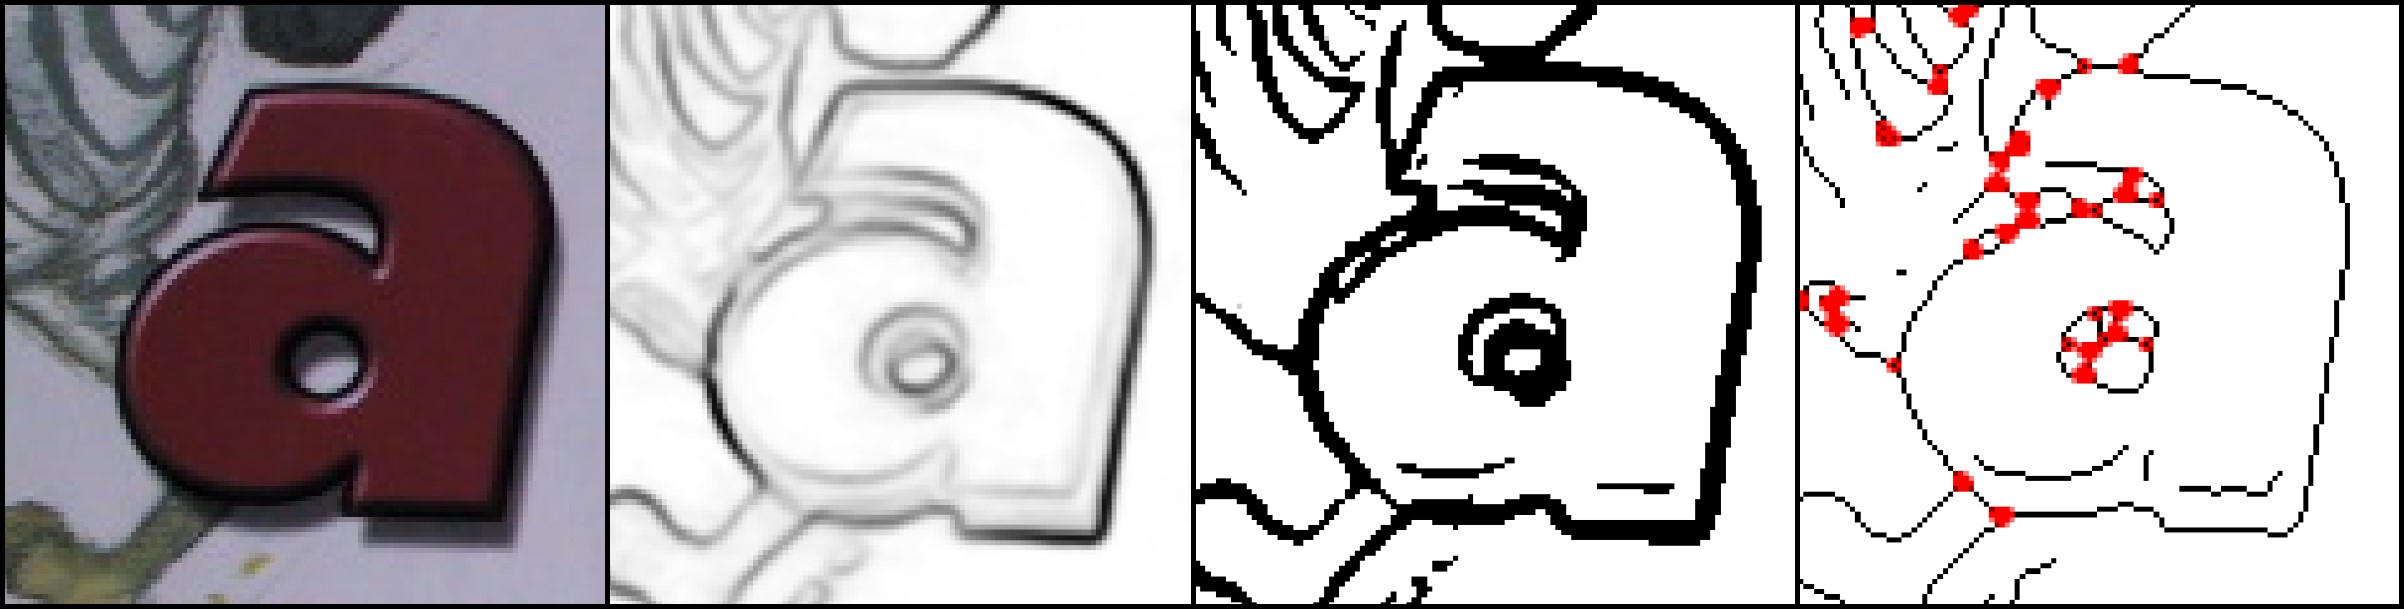
\includegraphics[width=\textwidth]{./figures/c3_skeleton.jpg}
        \begin{minipage}[t]{0.24\linewidth}
        \centerline{\small (a)原图}
        \end{minipage}
        \begin{minipage}[t]{0.24\linewidth}
        \centerline{\small (b)边缘响应}
        \end{minipage}
        \begin{minipage}[t]{0.24\linewidth}
        \centerline{\small(c)边缘二值图}
        \end{minipage}
        \begin{minipage}[t]{0.24\linewidth}
        \centerline{\small (d)边缘骨架图}
        \end{minipage}
        \caption{文字边缘骨架生成的流程图}
        \label{fig.c3_skeleton}
        \end{figure*}

        \subsection{文字骨架粘连点的检测和切割}
        \esubsection{Text adhesion-junctions' detection and cutting}
        \label{sec.c3_skeleton_cut}

        生成边缘骨架图后,就可以通过8连通区域的像素点数分析来检测边缘骨架粘连点。检测边缘骨架粘连点$J$的公式如下所示:

        \begin{equation}
        J=\left\{ p|n(p)=\sum_{k=1}^8x_k>t \right\},
        \label{eq:c3_junctions}
        \end{equation}
        
        在公式\ref{eq:c3_junctions}中,$n_p$是像素点$p$ 的8 连通区域内像素点的数目之和,而$t$ 是用来提取粘连点的像素点数目阈值。通过实验观察,令$t = 3$ 能检测到数目合适的候选边缘骨架粘连点,如图\ref{fig.c3_skeleton}中的红色结点所示。
        
        在\ref{sec.c3_skeleton}节中已经阐述,对于边缘响应图,利用不同的分割阈值可以得到相应的二值边缘图。而且分割阈值较大时,二值边缘清晰但粘连问题严重,阈值较小时非文字边缘大部分被消除但是文字边缘也出现断裂问题。因此选择合适的二值边缘图,使得既不会在图中出现过多的背景边缘,又能提供清晰的边缘信息,对后续解决边缘粘连问题至关重要。而观察由二值边缘图所生成的边缘骨架图的形态,就是一种判断所选边缘图是否合适的方式。

        \begin{figure}[htbp]
        \centering
        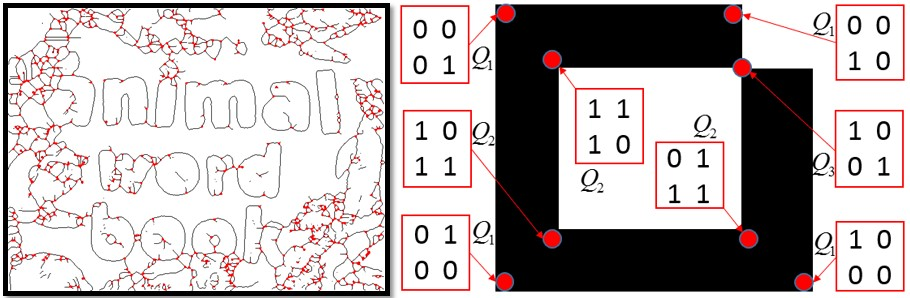
\includegraphics[width=\textwidth]{./figures/c3_select_skeleton.jpg}
        \begin{minipage}[t]{0.48\linewidth}
        \centerline{\small (a)无效的边缘骨架图}
        \end{minipage}
        \begin{minipage}[t]{0.48\linewidth}
        \centerline{\small (b)在边缘骨架图上计算欧拉数}
        \end{minipage}
        \caption{通过欧拉数的计算,选择出最合适的边缘骨架图}
        \label{fig.c3_select_skeleton}
        \end{figure}
        
        如图\ref{fig.c3_select_skeleton}(a) 所示,当分割阈值偏小时,从边缘响应图上分割得到的二值边缘图中混有过多的非文字边缘信息,因此通过细化操作所得的边缘骨架图十分杂乱无序,不能作为解决边缘粘连问题的有效信息。在这种混乱的边缘骨架图上检测到的候选边缘骨架粘连点,数目特别多且分布杂乱。因此,检测到的候选边缘骨架粘连点的数目,在一定程度上可以指示所选二值边缘图和相应的边缘骨架图的合理程度。除此之外,还可以通过对生成的边缘骨架图计算欧拉数,来避免选择不合适的边缘骨架图。

    \section{非文字骨架的滤除}
    \esection{Non-text skeleton's filtering}

        \subsection{形态学滤除}
        \esubsection{Morphological filtering}

        \subsection{基于卷积神经网络的滤除}
        \esubsection{convolutional neural network-based filtering}

    \section{文本行生成}
    \esection{Text line's construction}

        \subsection{最稳定极值区域的提取}
        \esubsection{Extraction of the most stable extremum region}

        \subsection{文本行的局部迭代优化}
        \esubsection{Text line's iteratively local refinement}

    \section{实验和结果分析}
    \esection{Experimental Results}

        \subsection{实验数据集与评价标准}
        \esubsection{Data-set and Evaluation Protocol}

        \subsection{实验结果与分析}
        \esubsection{Experimental Results and Analysis}

    \section{本章小结}
    \esection{Brief Summary}


